\section{Motivation}
{Die Ausgaben für das Internet der Dinge (IoT) wird weltweit, laut Statista, bis zum Jahr 2022 auf 1000 Milliarden US-Dollar steigen. Im Vergleich zum Jahr 2019 bedeutet dies, eine Steigerung von über 40\%.}\cite{STATISTA01:IOT} Bei einem solch starken Trend in der Informatik-Branche sollten sowohl Studenten, als auch Professoren dessen Grundlagen kennen.
Deshalb ist im Rahmen des Faches Softwarearchitektur an der technischen Hochschule Rosenheim diese Ausarbeitung geschrieben worden. Das Ziel ist es OpenHAB, ein Heimautomatisierungs-Tool, aus praktischer und technischer Sicht zu untersuchen. Außerdem wird dabei auf die Aspekte Markttauglichkeit und Benutzbarkeit in der Praxis eingegangen.

\section{Was ist OpenHAB?}
\label{s:what-is-openhab}
OpenHAB ist eine technologie-unabhängige Open-Source-Automatisierungssoftware für Smart-Homes.
Das Projekt wurde von Kai Kreuzer 2010 erstmals initiiert und wird mittlerweile durch die Community weiterentwickelt. Die Software ist hauptsächlich in Java und der Auszeichnungssprache XML geschrieben. Seit dem 16. Dezember 2019 ist die Version 2.5 erhältlich.\\
\\
Auf der offiziellen Website von OpenHAB \url{https://www.openhab.org/} sind drei klare Hauptziele definiert, die diese Software erreichen soll. Dabei ist ein Ziel die Plattformunabhängigkeit. Somit kann OpenHAB sowohl auf Linux, MacOS oder Windows betrieben werden. Auch das Hosten mit Docker oder einem Raspberry Pi wird unterstützt.\\
Weiterhin soll es durch die Plugin-Architektur möglich sein, fast jedes Gerät zu integrieren.
Es werden über 200 Technologien und mehrere tausende verschiedene Geräte unterstützt.\\
Das dritte Ziel weißt auf die vielen verschiedenen Automatisierungsmöglichkeiten hin, die OpenHAB zu bieten hat. Dabei werden Auslöser (in englisch: Trigger), Aktionen, Skripte und auch Voice-Kontrolle genannt.

\section{Bewertung OpenHAB}
In diesem Kapitel wird das open-source Projekt OpenHAB untersucht und bewertet. Es befindet sich auf Github unter \url{https://github.com/openhab/openhab-core}. Die hierfür verwendeten Kriterien sind orientiert an der QAware Open Source Quick-Check Liste.
Diese beinhaltet:
\begin{longtable}{| p{3cm} | p{12cm}|}
	\hline
	\textbf{Kriterium} & \textbf{Beschreibung} \\
	\hline \hline
	\centering Projekt Aktivität & Gibt es?
	\begin{itemize}
		\item Mindestens 1 Release im letzten Jahr
		\item Mindestens 3 aktive Contributer
		\item Stetige Commit-Aktivität von mindestens 1x pro Monat
	\end{itemize}\\
	\hline
	\centering Reifegrad & Existiert eine stabile Version > 1.0?  \\
	\hline
	\centering Lizenz & Für welche Zwecke kann das Projekt genutzt werden? \\
	\hline
	\centering Support & Existiert Issue-Tracking und ein Antwortzeit auf Tickets unter 24h? \\
	\hline
	\centering Dokumentation & Existiert?
	\begin{itemize}
		\item Api-Dokumentation
		\item Getting Started Tutorial
		\item Aktuelle Dokumentation
	\end{itemize} \\
	\hline
	\caption{OpenHAB Projektbewertungskriterien}
	\label{table:openhab-judgement-criteria}
\end{longtable}

Der Online-Dienst \textbf{Open Hub}, ehemals \textbf{Ohloh} genannt, katalogisiert opensource Softwareprojekte. Dabei werden Daten wie Projektname, Beschreibung und Sourcecode erfasst. Basierend auf diesen Daten erstellt Open Hub eine Statistik, die es ermöglicht, Codeanalyse, Projektmitarbeiter, Aktivitäten und eine Übersicht zu erhalten. Dabei werden auch viele weitere open source Projekte miteinander verglichen um aussagekräftige Statistiken und Aussagen treffen zu können.\\
\\
{In der Auswertung über OpenHAB steht beispielsweise, dass im letzten Jahr 343 Entwickler aktiv an dem Projekt mitgearbeitet haben. Somit ist OpenHAB unter den top 2\% der größten Projektteams auf Open Hub.\\
Des Weiteren ist ein stetiger Anstieg von Interesse erkennbar. Dies wird durch den Vergleich von Codebeiträgen des aktuellen Jahrs und des Vorjahres begründet.\\
Insgesamt haben über 1140 Entwickler bereits mehr als 20000 Beiträgen in Form von Programmcode zum Projekt beigetragen. Der Umfang des zu 98\% in Java geschriebenen Codes beträgt mehr als 1.5 Millionen Zeilen. Davon wurden circa 31\% dokumentiert. Dies entspricht dem durchschnittliche Wert aller Java open-source Projekte, welche auf Open Hub registriert sind.}\cite{OPENHUB01:OH} Die hierbei angegeben Werte beziehen sich auf alle Projekte und Subprojekte von OpenHAB. Eine Übersicht hierfür ist unter \url{https://github.com/openhab} zu finden.\\
\\
Wie bereits im Kapitel \ref{s:what-is-openhab} erwähnt, ist OpenHAB aktuell in der Version 2.5 erhältlich. Daraus lässt sich auf einen stabilen Codestand schließen.\\
Des Weiteren ist das Projekt unter einer EPL-2.0 Lizenz veröffentlicht. Dies erlaubt sowohl die private als auch kommerzielle Nutzung. Hinzu kommt die Möglichkeit für Modifizierung und Weiterverbreitung.\cite{LICENSE01:EC}
\\
\\
Des Weiteren wird die Qualität des Supports evaluiert. Hierfür stellt Github einen Issue-Tracker zur Verfügung. Beim Teilprojekt openhab-core wurden darüber über 1250 Issues verfasst, wovon bei circa 90\% bereits die Bearbeitung abgeschlossen ist.\cite{GITHUB01:OS} Dies lässt auf eine aktive Nutzung des Issue-Trackers schließen und bietet somit eine hilfreiche Support-Möglichkeit. Hierfür ist vor allem das Label \textbf{Bug} von Bedeutung. Eine Stichprobenartige Untersuchung von Issues dieses Types hat eine durchschnittliche Antwortzeit in unter 24h ergeben. Dies wurde anhand des ersten Kommentars gemessen. Zudem wurden bereits circa 83\% der insgesamt 68 dokumentierten Bugs gelöst.
\\
\\
Abschließend wird der Zustand der Dokumentation untersucht.
Das Getting-started Tutorial ist ausführlich und aktuell. Die darüber hinausgehende Basisdokumentation ist vollständig. Nur in Spezialfällen, wie beispielsweise der Implementierung von Services, ist die Dokumentation lückenhaft.\cite{OPENHAB01:OH}

\subsection{Fazit der Bewertung}
\begin{longtable}{| p{3cm} | p{10cm}| c |}
	\hline
	\textbf{Kriterium} & \textbf{Beschreibung} & \textbf{Erfüllt?} \\
	\hline \hline
	\centering Projekt Aktivität & Gibt es?
	\begin{itemize}
		\item Mindestens 1 Release im letzten Jahr
		\item Mindestens 3 aktive Contributer
		\item Stetige Commit-Aktivität von mindestens 1x pro Monat
	\end{itemize} & \checkmark \\
	\hline
	\centering Reifegrad & Existiert eine stabile Version > 1.0? & \checkmark \\
	\hline
	\centering Lizenz & Für welche Zwecke kann das Projekt genutzt werden? & \checkmark \\
	\hline
	\centering Support & Existiert Issue-Tracking und ein Antwortzeit auf Tickets unter 24h? & \checkmark \\
	\hline
	\centering Dokumentation & Existiert?
	\begin{itemize}
		\item Api-Dokumentation
		\item Getting Started Tutorial
		\item Aktuelle Dokumentation
	\end{itemize} & X/\checkmark \\
	\hline
	\caption{OpenHAB Projektbewertungskriterien Ergebnis}
	\label{table:openhab-judgement-criteria-result}
\end{longtable}

\subsection{Weiterführende Bewertungen}
OpenHAB wurde bereits in der Bachelorarbeit von Pirmin Gersbacher vom Jahr 2017/2018 anhand von Usecases untersucht und verglichen. Dabei kam er zu folgender Ergebnis.

\begin{minipage}{\textwidth}
	\centering
	\captionsetup{type=figure}
	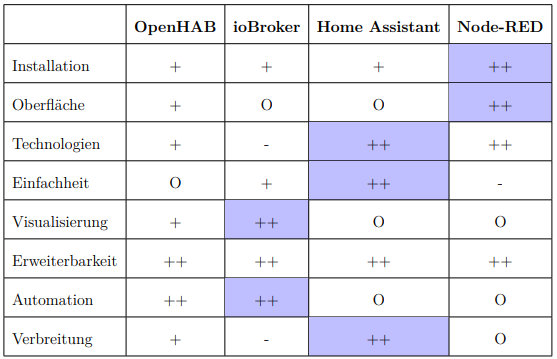
\includegraphics[width=0.8\textwidth]{\figdir/comparison-openhab.PNG}
	\caption{Vergleich OpenHAB und anderen Heimautomatisierungstools von 2017/2018 \label{fig:comparison-openhab}}
\end{minipage}

In der Tabelle \ref{fig:comparison-openhab} sind die unterschiedlichen Gebiete der Untersuchung auf der linken Seite zu finden. In der horizontalen sind die einzelnen Heimautomatisierungs-Tools aufgelistet. In der jeweiligen Zelle, basierend auf Reihe und Spalte, sind die Bewertungen festgehalten. Dabei zeigt ein blau markiertes Feld, welches das beste Tool für ein Gebiet ist.\\
OpenHAB sticht dabei nicht sonderlich heraus. Allerdings ist es in keinem der aufgelisteten Kategorien negativ bewertet.\\
Der Autor schreibt in seiner Bachelorarbeit, dass er persönlich auf OpenHAB setzen würde. Dies liegt einerseits daran, dass die Entwickler von OpenHAB stark an Vereinfachung von komplizierteren Komponenten arbeitet. Andererseits sollen aber auch komplexere Automationen, durch die Nähe von Framework und Java, möglich sein.\cite{BA01:OPH}


\section{Datenintegriertät und Sicherheit}
\url{https://www.openhab.org/docs/installation/security.html}
\begin{itemize}
	\item Through the command line console, which is done through SSH and thus always authenticated and encrypted. You will find all details about this in the Console documentation.
	\item Through HTTP(S) over \url{https://<ip>:8443}
	\item Options for Secure Remote Access
	\begin{itemize}
		\item VPN: The most secure option is probably to create a VPN connection to your home network
		\item myopenHAB Cloud Service with a tunnel that forwards all requests to the openHAB instance
		\item Running openHAB Behind a Reverse Proxy: A reverse proxy simply directs client requests to the appropriate server. This means you can proxy connections to \url{http://mydomain_or_myip} to your openHAB runtime.
	\end{itemize}
\end{itemize}



\section{openHAB aus technischer Sicht}
In diesem Kapitel werden die grundlegenden Komponenten welche openHAB verwendet dargestellt. Des Weiteren wird auf die  Beziehung der Komponenten untereinander eingegangen. 
Es wird ein Kern Aspekt von openHAB vorgestellt. openHAB bietet in der Regel nicht den "einen Weg". Es bietet mehrere Wege ein Ziel zu erreichen, je nach Vorlieben des Nutzers. So ist es z.B. möglich ein Gerät über die Web-Oberfläche als auch über geschriebenen Code zu integrieren. Das gleiche ist auch bei Rules zu sehen, welche entweder über ein Add-on in der Web-Oberfläche definiert werden können, oder über Code. Dieses Konzept ist ein Grundgedanken, welcher von openHAB verfolgt wird, welcher allerdings zu Verwirrung führen kann, da bei anfänglichen Umgang mit openHAB nicht unbedingt klar ist, wie man sein gewünschtes Ziel erreichen kann.
In \ref{table:openhub-components} sind einige der Grundlegenden Komponenten aus openHAB zur schnellen Übersicht aufgeführt. Detailliert werden diese in den Entsprechenden Unterkapiteln beschrieben.

\begin{longtable}{| p{5cm} | p{10cm}|}
	\hline
	\textbf{Komponente} & \textbf{Beschreibung} \\
	\hline \hline
	\centering Add-ons & Erweiterungen, welche die Funktionalitäten von openHAB erhöhen. \\
	\hline
	\centering Bindings & openHAB-Komponenten, welche die Schnittstelle zu fremd Systemen darstellt.  \\
	\hline
	\centering Things & Repräsentation von physischen Geräten in openHAB. \\
	\hline
	\centering Items & Darstellung von Eigenschaften und Ressourcen von openHAB - Thing bezogen \\
	\hline
	\centering Channels & Übertragungskanal zwischen "`Items"' und "`Things"'. \\
	\hline
	\centering Rules & Automatisierungsregeln, in Wenn-Dann-Struktur.\\
	\hline
	\centering Sitemaps & individuelle Benutzeroberfläche, welche Informationen präsentiert und Interaktionen ermöglicht.\\
	\hline
	\caption{OpenHAB Komponenten}
	\label{table:openhub-components}
\end{longtable}

\subsection{Add-ons}
openHAB sich selbst als System bezeichnet welches alles Integriert, dies wird dadruch erreicht, dass es von der so konzipiert ist, dass bestimmte bereiche jederzeit erweitert werden können. OpenHAB gibt hier als verschiedene Module/Komponenten, welche neu hinzugefügt werden können vor.
\begin{itemize}
	\item Bindings
	\item Automation Engine Modules
	\item Transformations / Profiles
	\item IO Services
	\item Persistence Services
	\item Audio \& Voice
\end{itemize}
Um nicht den Rahmen dieser ARbeit zu übersteigen wird Detailierter auf Bindings eingegangen. Was unter anderem daran liegt, dass Die Dokumentation von openHAB, welche die entwicklung von IO-, Persistence Services und Audio/Voice mit einem TODO beschreibt eher dürftig ist. Bei den Transforamtions / Profiles handelt es sich um transformationen welche genutzt werden können um zu übertragenede Werte durch einen Channel zu manipulieren/tranformieren.
Add-ons sind in openHab das Herzstück der pluggable Architecture. Da Nutzer des Systems ihre individuellen Bedürfnisse haben und sich demnach nciht alle verfügbaren Add-ons installieren müssen, sondern nur diejenigen welche für Ihre Bedürfnisse nötig sind. Sollte es allerdings keine passendes Add-on für ein gewünschtes Gerät geben, steht der erweituerng und dem entwicklen eines eigenenen Add-ons durch das Add-on System nichts im Weg. Mehr noch, durch den OpenSource gedanken, welcher openHAB vorantreibt könnte das Gesamt-System durch ein weiteres Add-on erweitert werden. 

\subsection{Bindings}
Bindings sind die Schnittstelle bzw. die Erweiterung, welche es erst ermöglicht andere Systeme mit openHAB zu integrieren. Mit einem Binding kann sowohl ein Pysisches Geräte z.B. eine LG Fernseher als auch eine Service z.B. Spotify angebunden werden. Die Bindings sind dabei soweit abstrahiert, dass nicht jedes einzelne Model bzw. Version eine eigenes Binding benötigt.
Ein Binding ermöglicht es dem System erst neue Geräte im System zu erkennen. Und diese als Thing im openHAB System zur weiteren Interaktion zur Verfügung zu stellen. Interessant ist hierbei, dass Bridges oder Schnittstellen wie Bluetooth es erst ermöglichen Weitere Geräte zu erkennen. So kann durch das Hue-Binding die Hue-Bridge integriert werden, welche es wiederum ermöglicht einzelne Komponenten des Hue-Systems anzusprechen (Lampen), welche nicht direkt erkannt und angesporchen werden konnten.
Laut openHAB gibt es aktuell über 300 Bindings und dadurch können über 2000 Things angesprochen werden.
OpenHab bietet zusätzlich zur Dokumentation noch Untestützung für das Entwickeln eines Eigenen Bindings durch eine Skeletton skript, welches die Stuktur eines Bindings inklusive Beispielen und Erklärungen welche Methonde/Funktionen wie gestaltet werden müssen und was diese Tun. Siehe:
\captionsetup{type=figure}
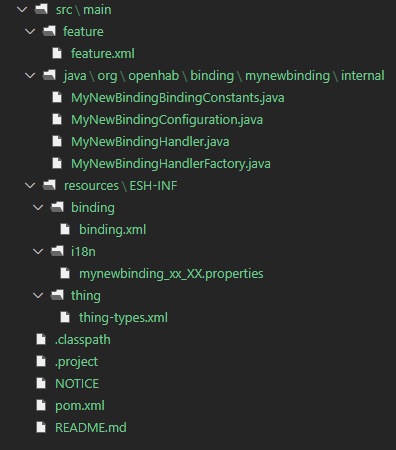
\includegraphics[width=0.5\textwidth]{\figdir/own_binding_skeletton.PNG}
\caption{Skelett für Binding \label{fig:own_binding_skeletton}}


\subsection{Things}
Things sind die repräsentation von Geräten/Services innerhalb des Systems. Berachtet man die Objektorierntierung ist es ein sehr schönes Beispiel wie im einem Computersystem ein realer gegenstand beschreiben werden kann.
Things bieten verschiedene so gennante Channels an. Diese entsprechen die Funktionen/Aktionen welche das Gerät ausführen kann.
Things können auf 3 verschiedene arten openHAB hinzugefügt werden
\begin{itemize}
	\item per Web-Oberfläche per Button click in der Inbox, nachdem das entsprechende Binding installiert wurde. Hierbei werden alle nötigen Einstellungen für das Thing automatisch getroffen. Diese können nachträglich noch bearbeitet werden z.B. Bezeichnung. 
		\captionsetup{type=figure}
		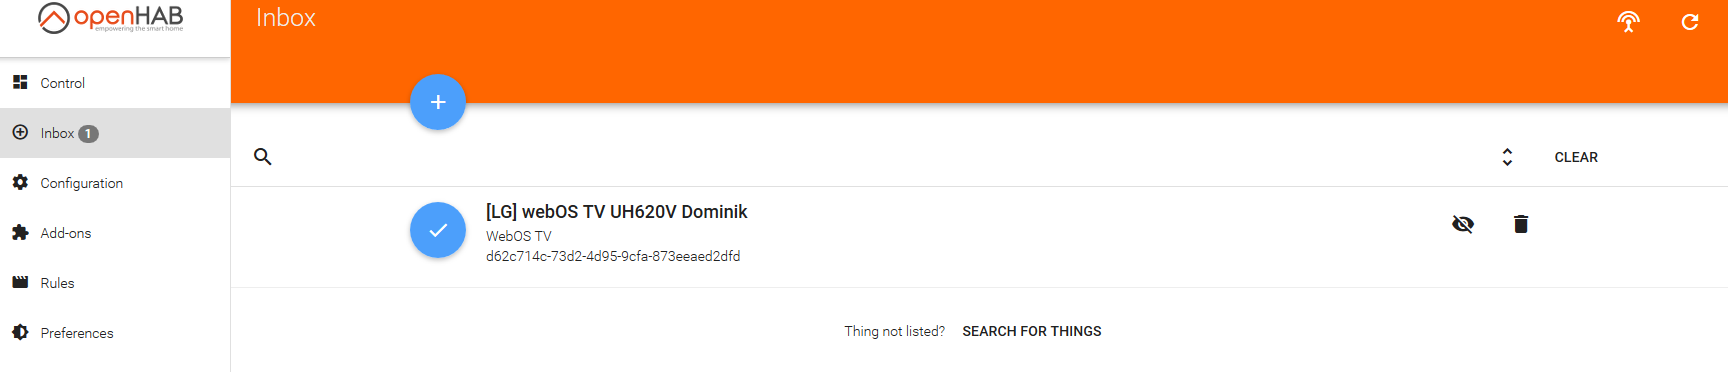
\includegraphics[width=1\textwidth]{\figdir/thing_add.PNG}
		\caption{Thing per Paper-UI \label{fig:thing-add-paper-ui}}
		
	\item per Web-Oberfläche Manuell. Erlaubt völlige Einstellung im Vorhinein. Allerdings ist auf Statische IP-Adressen zu achten.
		\captionsetup{type=figure}
		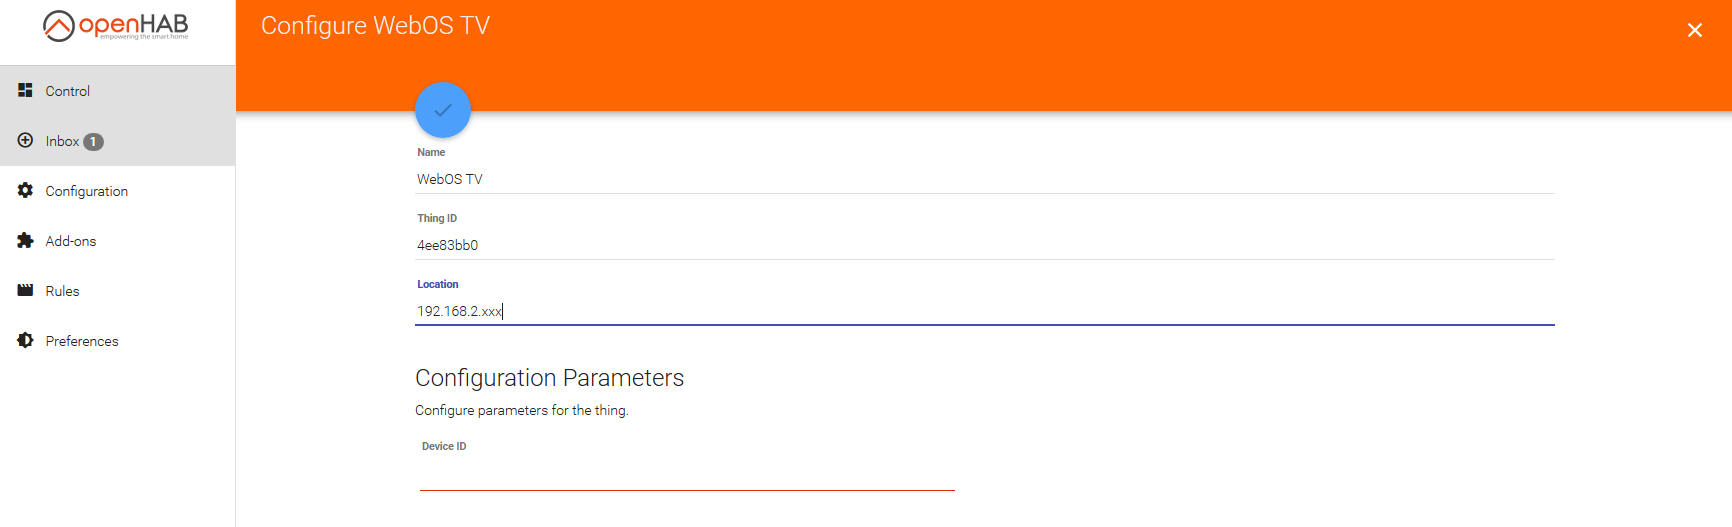
\includegraphics[width=1\textwidth]{\figdir/thing_add_manuel.PNG}
		\caption{Thing per Paper-UI Manuell \label{fig:thing-add-paper-ui-manuel}}
		
	\item per Code. Ermöglicht und benötigte komplette manuelle eingabe aller nötiger Infomrmationen wie IP-Adresse
		\captionsetup{type=figure}
		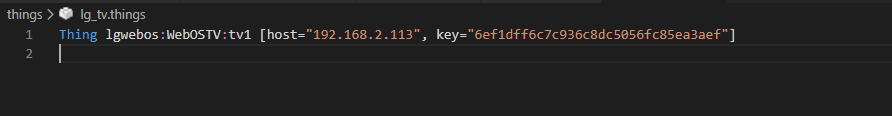
\includegraphics[width=1\textwidth]{\figdir/thing_add_code.PNG}
		\caption{Thing per Code \label{fig:thing-add-code}}
\end{itemize}

\subsection{Channels}
sind Kommunikationswege welche von den Things angeboten werden. Channels verbinden Things und Items. Und könne in openHab, bzw. den Rules genutzt werden. Sie stellen die Verbindung von externen Gerät zu openHAB aktionen dar. Über die Channels können Informationen durch PAramerter ausgetauscht werden. So wäre z.B. die Helligkeit einer Lampe ein Parameter, welcher durch einen Channel übertragen werden kann. nicht jedoch die Informationen, dass sich die Helligkeit ändern soll. Hierfür wird das Item benötigt, welches durch den Channel an das Thing verbunden wrude.

\subsection{Items}

Der Begriff Item wirkt unter umständen falsch. Ein Item könnte auch als Aktion beschreiben werden. Ein Item selbst hat sehr wenig Informationen. Das Item besteht neben eine Titel noch aus eine Kategorie und eine Gruppe um es zuzuordnen und um gleichzeitig mehrere Items gleichzeitig anzusteueren.. Außerdem hat ein Item noch einen Typ, dieser Typ entspricht einer Menge von Basistypen, welche von openHAB angeboten werden. Diese sind unter anderem String, Numnber, DateTime, Location, Player usw. \url{https://www.openhab.org/docs/configuration/items.html#type}.
Wichtig ist auch der Status. Wodoruch es doch wieder ein Item anstatt einer Aktion ist. (könnte man item als object bezeichnen mit label, kategorie, status und nur einer funktion??? memo an mich DAM)
Items sind essentielle bestandteile um das Panel zu bauen, da die Widgets über Items mit den Geräten agieren.
so schaut ein item aus  

jedes item einen channel zugeordnet. 
\begin{lstlisting}[language=java,firstnumber=1,caption=Item Beispiel,label=lst:sample-item]
{
	"type": "string",
	"name": "string",
	"label": "string",
	"category": "string",
	"tags": [
	"string"
	],
	"groupNames": [
	"string"
	],
	"link": "string",
	"state": "string",
	"transformedState": "string",
	"stateDescription": {
		"minimum": 0,
		"maximum": 0,
		"step": 0,
		"pattern": "string",
		"readOnly": false,
		"options": [
		{
			"value": "string",
			"label": "string"
		}
		]
	},
	"metadata": {},
	"editable": false
}
]
\end{lstlisting}

\begin{lstlisting}[language=java,firstnumber=1,caption=Item-Gruppierung Beispiel,label=lst:group-items]
	Group groundFloor
	Switch kitchenLight (groundFloor)
	Switch livingroomLight (groundFloor)
\end{lstlisting}

\subsection{Link}

\subsection{Rules}
Automatisierung wir durch Rules/Scripte erreicht, welche in erster linie durch Programmieren erzeugt werden. Um Regeln zu erzeugen, wird eine einfache wenn/dann-Struktur verwendet. Diese Regeln können auf verschiedene Bedingungen "lauschen". So können die Trigger von Items, Member of, Time, System oder Things stammen. Genauer kann die Bedingung noch durch eine verschiedene Formen eingeschränkt werden wie z.B. received command [<command>],  received update [<state>] oder changed [from <state>] [to <state>] usw.
Wenn diese Bedingung erfüllt ist, wird im DANN-Pfad die Reaktion definiert. So können Item oder Ganze Gruppen angesprochen werden und durch diese über Channels Informationen weitergegeben werden.
Wie im Codebeispiel 2?? zu sehen, kann auch innerhalb dies Then-Blocks weitere Sturkturelemente eingefügt werden um z.B. aus mehrerern Rules eine zu maer Arbeit können dadurch scheon (wie im Beispiel)

Alternativ zum Programmieren gibt es ein experimentelles Add-on, welches es über die Paper-UI ermöglicht Regeln zu definiert werden. Allesrdings ist hier anzumerken, dass Komplexere Regeln schwierig bis garnicht zu erzeugen sind. Dies liegt waran, dass die eingabeparameter und JSON-Format gespeichert werden und durch die konvertierung des formates sonderzeichen und komplexe strukturen schwierig bis garnicht übertragen lassen.

Codeblock \ref{lst:sample-rule} zeigt ein programmatisch erstellte Rule.
\begin{itemize}
		\item Eine Rule besteht immer aus einem Namen, einer when-Bedinung und einem then Abschnitt.
		\item Name dient als Zuordnung
		\item When ist der Trigger bzgw. Auslöser der Aktion, welche im then Block definiert ist.
		\item Diese Rule prüft, ob die Lautstärke des Items (TV) Dominik\_volumen sich verändert hat.
		Wenn das der Fall ist, wird eine geprüft, wiehoch denn die aktuelle Lautstärke ist.
		Folglich wird bei unter 20 die Lampe gedimmt und bei über 20 die Lampe erhellt.
		\item Falls etwas nicht klappen sollte, können auch Debug-Ausgaben mit dem Kommando logDebug geschrieben werden.
\end{itemize}

\begin{lstlisting}[language=java,firstnumber=1,caption=Beispiele Rule Beispiel,label=lst:sample-rule]
rule "React on Volume (LGWebOSTVUH620VDominik_Volume) change"
when
	Item LGWebOSTVUH620VDominik_Volume changed
then
	logDebug("React some changes on Volume", "some Message" + LGWebOSTVUH620VDominik_Volume.state.toString)
if ( LGWebOSTVUH620VDominik_Volume.state >= 20 ) {
	HueWhiteLamp2_Brightness.sendCommand(80)
}
else {
	HueWhiteLamp2_Brightness.sendCommand(5)
}
end
\end{lstlisting}

\subsection{Sitemaps}
Sitemaps dienen als Übersicht, Gruppierung und Visualisierung des Smart-Homes. So werde durch Sitemaps räume nachbildet um Komplette beleuchtung innerhalb eines Raums ein/auszuschalten, Temperatur o.ä. im Auge zu behalten. Neben Sitemaps können auch ander Darstellung wie Panels verwendet werden. SiteMap und Dashboards dienen wie der Name schon sagt als Dashboard (Wie blöd kann ich denn das schreiben). Und als kontrolleinheit für das Smart-Home. Die Erstellung wird durch eiditoren errleichtert, welche Programmierunkundigen Code-Snippits zur Verfüfung stellt.

\subsection{Api}
OpenHAB nutzt um die Paper-UI zu nutzen eine REST-API. Diese ist offengelegt, was anderen Systemen es ermöglicht die Komplette Funktionalität, welche über die Web-Oberfläche nutzbar ist ebenfalls zu integrieren. Dies ermöglicht es unter anderem Entwicklungsumgebungen wie VS-Code, Eclipse, IntelliJ Add-Ons/Extensions zu entwickeln, welche das Prgrammieren für OpenHab vereinfacht. So bieten diese 3 Extensions welche die Rest-Api nutzen um ITEMS und Things welche im System verfügbar sind anzuzeigen, was es sehr angenehm macht Rules o.ä. zu entwickeln.
Die Rest-API ermöglicht es ebenfalls unabhänigen entwicklern openHAB funktionen zu steuern, was allerdings im Mobilen bereich irrelevant sein sollte, da es android, ios und windows apps bereits gibt


\subsection{Entwickeln für OpenHAB??}

OpenHAB liefert für das Entwickeln von Add-Ons Skelleton-Skripte, welche die von openHAB bentigte Struktur erzeugen. Für manuelles Hinzufügen von Things, Items, Rules usw. bietet openHAB bereits eine ORdnerstruktur. Diese ist so offensichtlich, dass es trivial ist zu entscheiden, wo welche Komponente hinzugefügt werde soll. Sollte dies dennoch unklar sein, wird der Nutzer noch weiter durch readme-dateien unterstützt. Siehe 


\captionsetup{type=figure}
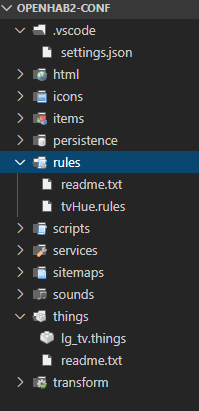
\includegraphics[width=0.25\textwidth]{\figdir/openHab-conf-folder-structure.PNG}
\caption{openHAB-conf Ordnerstruktur \label{fig:openHab-conf-folder-structure}}



ich muss mir noch überlegen, ob ich daraus ein eigenes kapitel mach, oder ob e sunter die anderen bauch.
\url{https://www.openhab.org/docs/configuration/restdocs.html}
\begin{itemize}
	\item Item ein-/ausschalten
	\item Eine List von allen Items, Sitemaps ausgeben lassen
	\item Mit einem Editor auf die ganzen Komponenten zugreifen:
	\begin{itemize}
		\item Visual Studio Code installieren
		\item Openhab Extension installieren
		\item Geteiltes Openhab Laufwerk als Ordner öffnen
		\item Openhab Extension konfigurieren
		\item Es werden auch andere Editoren unterstützt
	\end{itemize}
\end{itemize}

\section{Verwendung von OpenHAB}
\subsection{Integration der Big Player}
\begin{itemize}
	\item Amazon Alexa und Echo Dot Integration möglich
	\begin{itemize}
		\item Alexa:
		\begin{itemize}
			\item This certified Amazon Smart Home Skill allows users to control their openHAB powered smart home with natural voice commands. Lights, locks, thermostats, AV devices, sensors and many other device types can be controlled through a user's Alexa powered device like the Echo or Dot.
			\item \url{https://www.openhab.org/docs/ecosystem/alexa/}
			\item \url{https://www.openhab.org/addons/bindings/amazonechocontrol/}
		\end{itemize} 
		\item Google Home
		\begin{itemize}
			\item Google Home Integration möglich
			\item With the Action you can voice control your openHAB items and it supports lights, plugs, switches and thermostats. The openHAB Action comes with multiple language support like English, German or French language.
			\item The openHAB Action links your openHAB setup through the myopenHAB.org cloud service to the Google Assistant platform
			\item openHAB Cloud Connector configured using myopenHAB.org . (Items DO NOT need to be exposed to and will not show up on myopenHAB.org
			, this is only needed for the IFTTT service!)
			Google account.
			Google Home or Google Home mini.
			
			\url{https://www.openhab.org/docs/ecosystem/google-assistant/}
		\end{itemize} 
	\end{itemize}
	
\end{itemize}

\subsection{Beispiel Aufbau eines OpenHAB Smart-Homes}
\begin{itemize}
	\item OpenHAB auf Raspberry Pi 3/4 installiert
	\item Welche Geräte haben wir mit OpenHAB verbunden?
	\begin{itemize}
		\item Spotify
		\begin{itemize}
			\item Lautstärkeregler
			\item Aktueller Song Display
		\end{itemize}
		\item LG Smart TV
		\begin{itemize}
			\item Lautstärkeregler
			\item An- und ausschalten
			\item One-Way-Chat
		\end{itemize}
		\item Lampen
	\end{itemize}
	\item Wie haben wir die Geräte verbunden?
	\begin{itemize}
		\item \textbf{Verschiedene Binding:}
		\item Spotify Binding
		\item LG Smart TV Binding
	\end{itemize}
	\item On the server the configuration is stored somewhere in userdata (/var/lib/openhab2 for apt-get installs).
	In an upgrade the userdata folder is preserved when using apt-get.
\end{itemize}
\begin{minipage}{\textwidth}
	\centering
	\captionsetup{type=figure}
	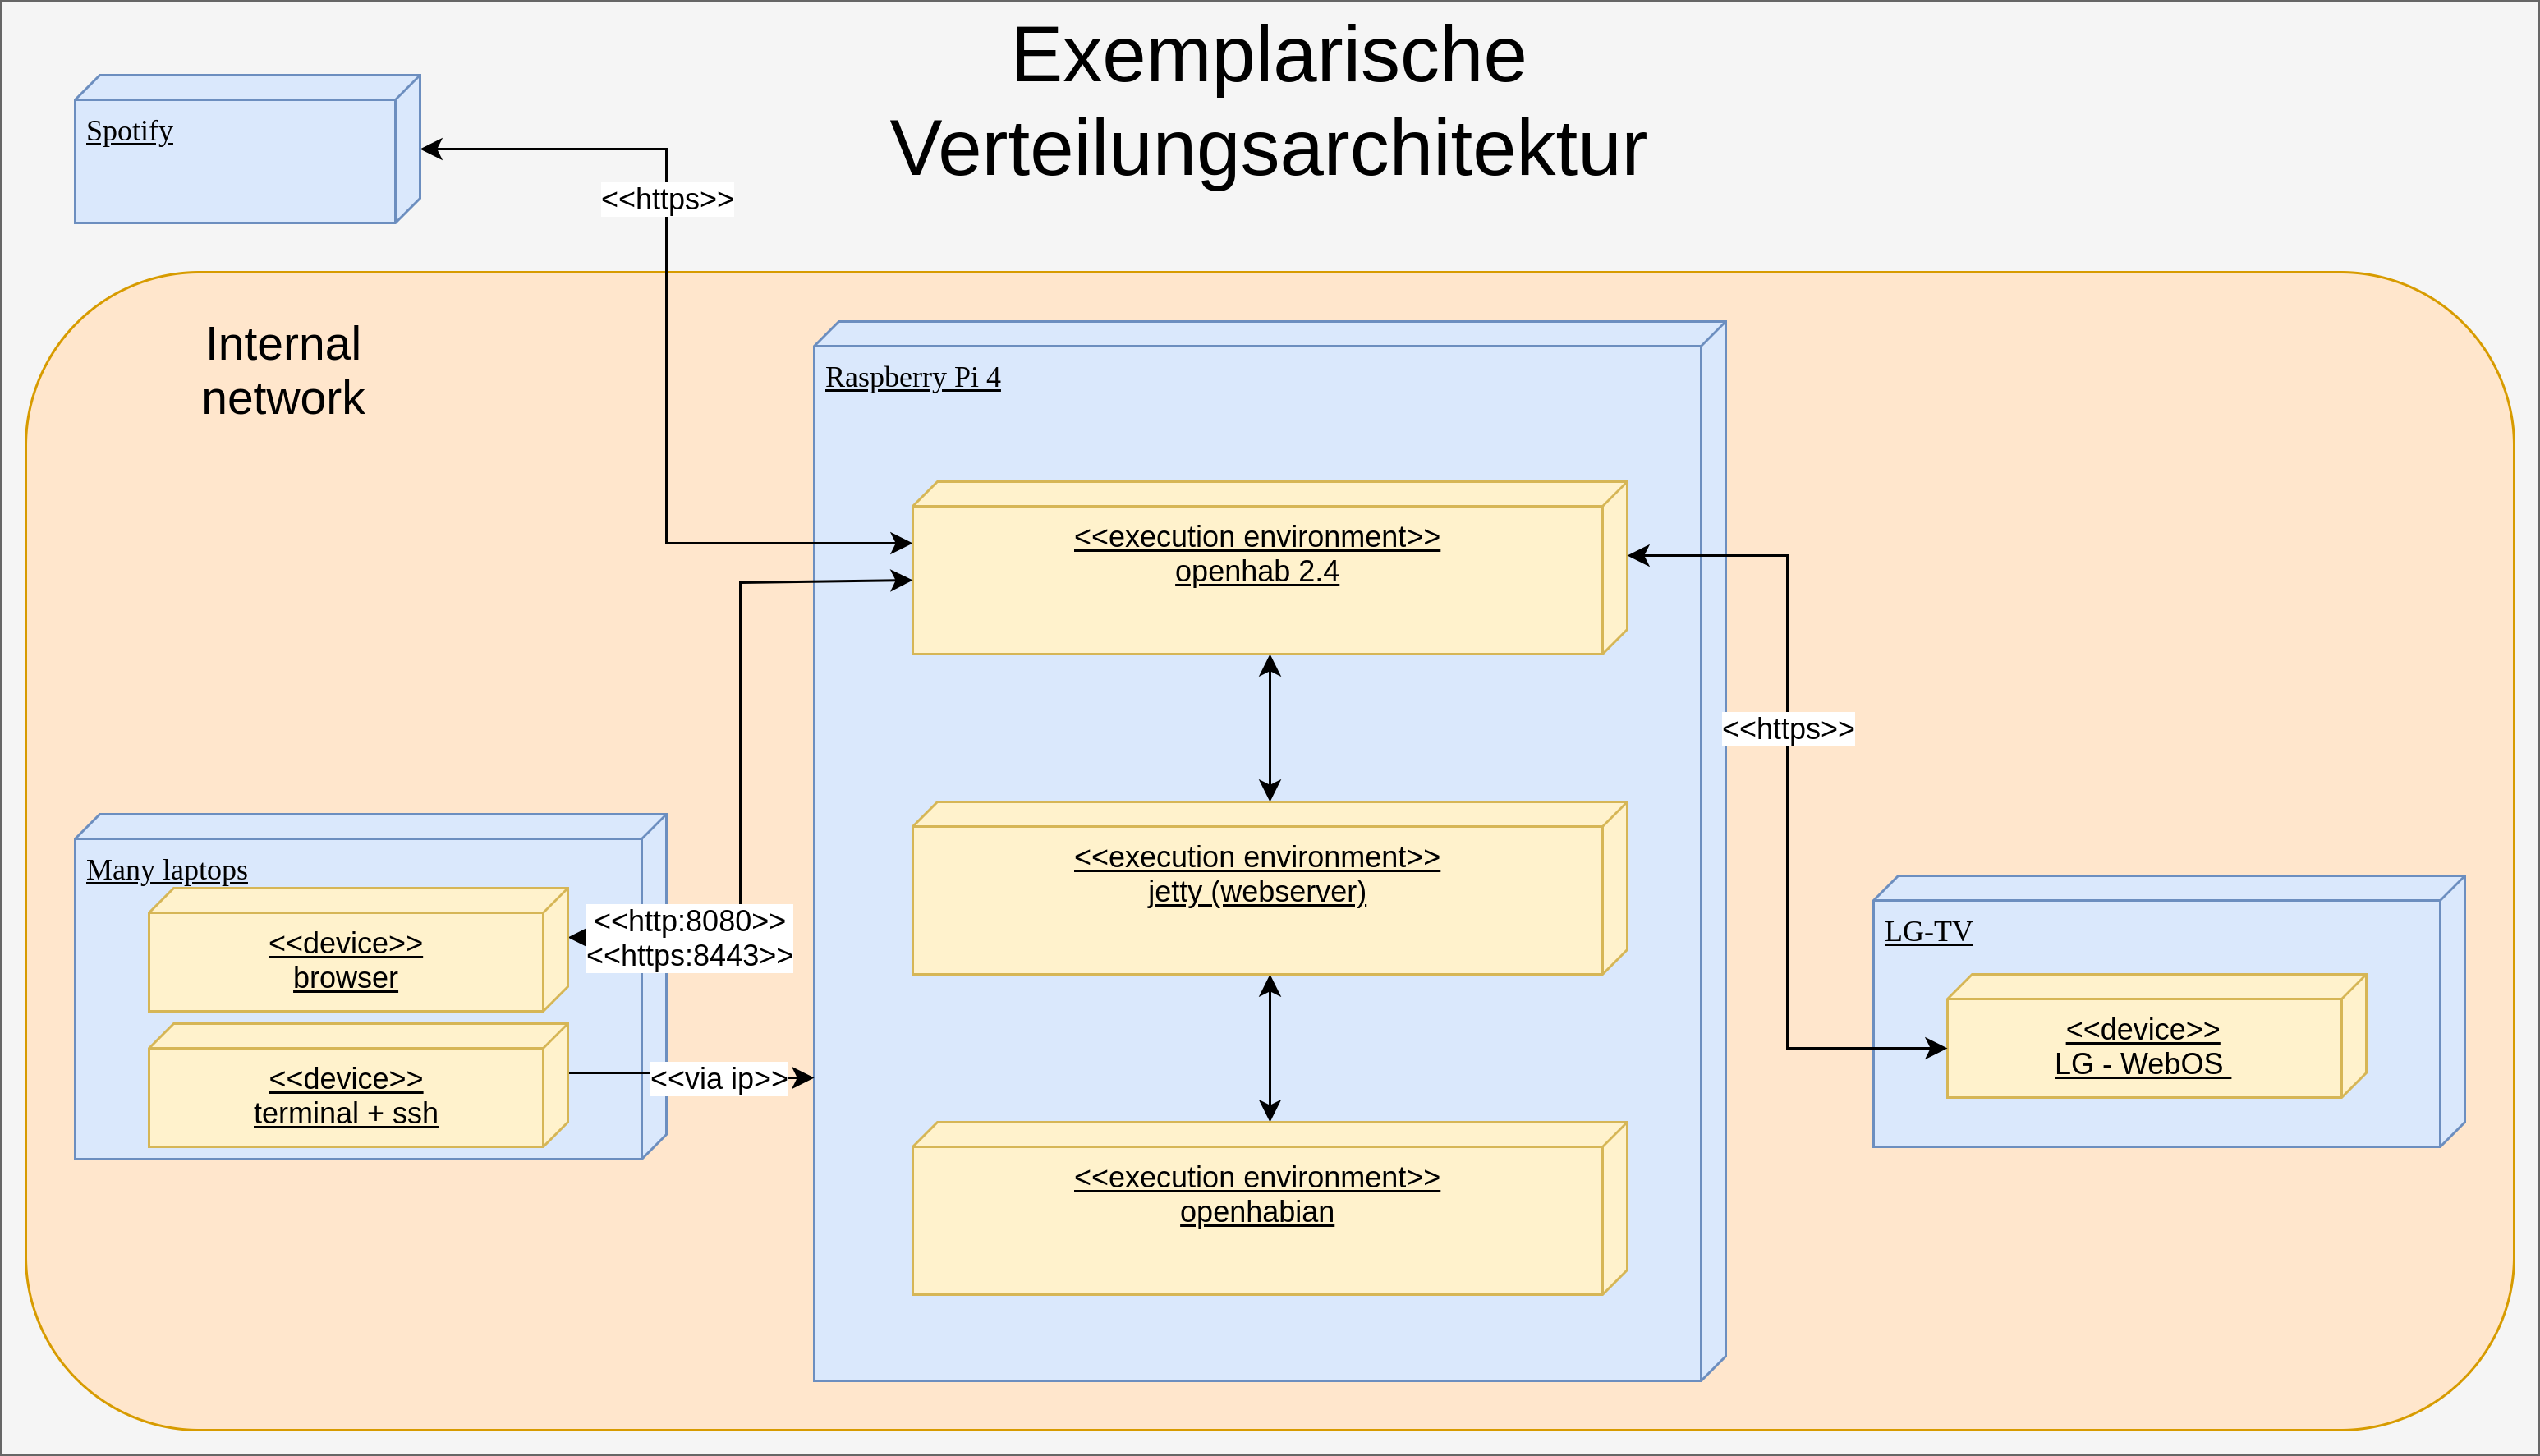
\includegraphics[width=1\textwidth]{\figdir/verteilungsarchitektur.png}
	\caption{Verteilungsarchitektur \label{fig:verteilungs-architektur}}
\end{minipage}
\begin{minipage}{\textwidth}
	\centering
	\captionsetup{type=figure}
	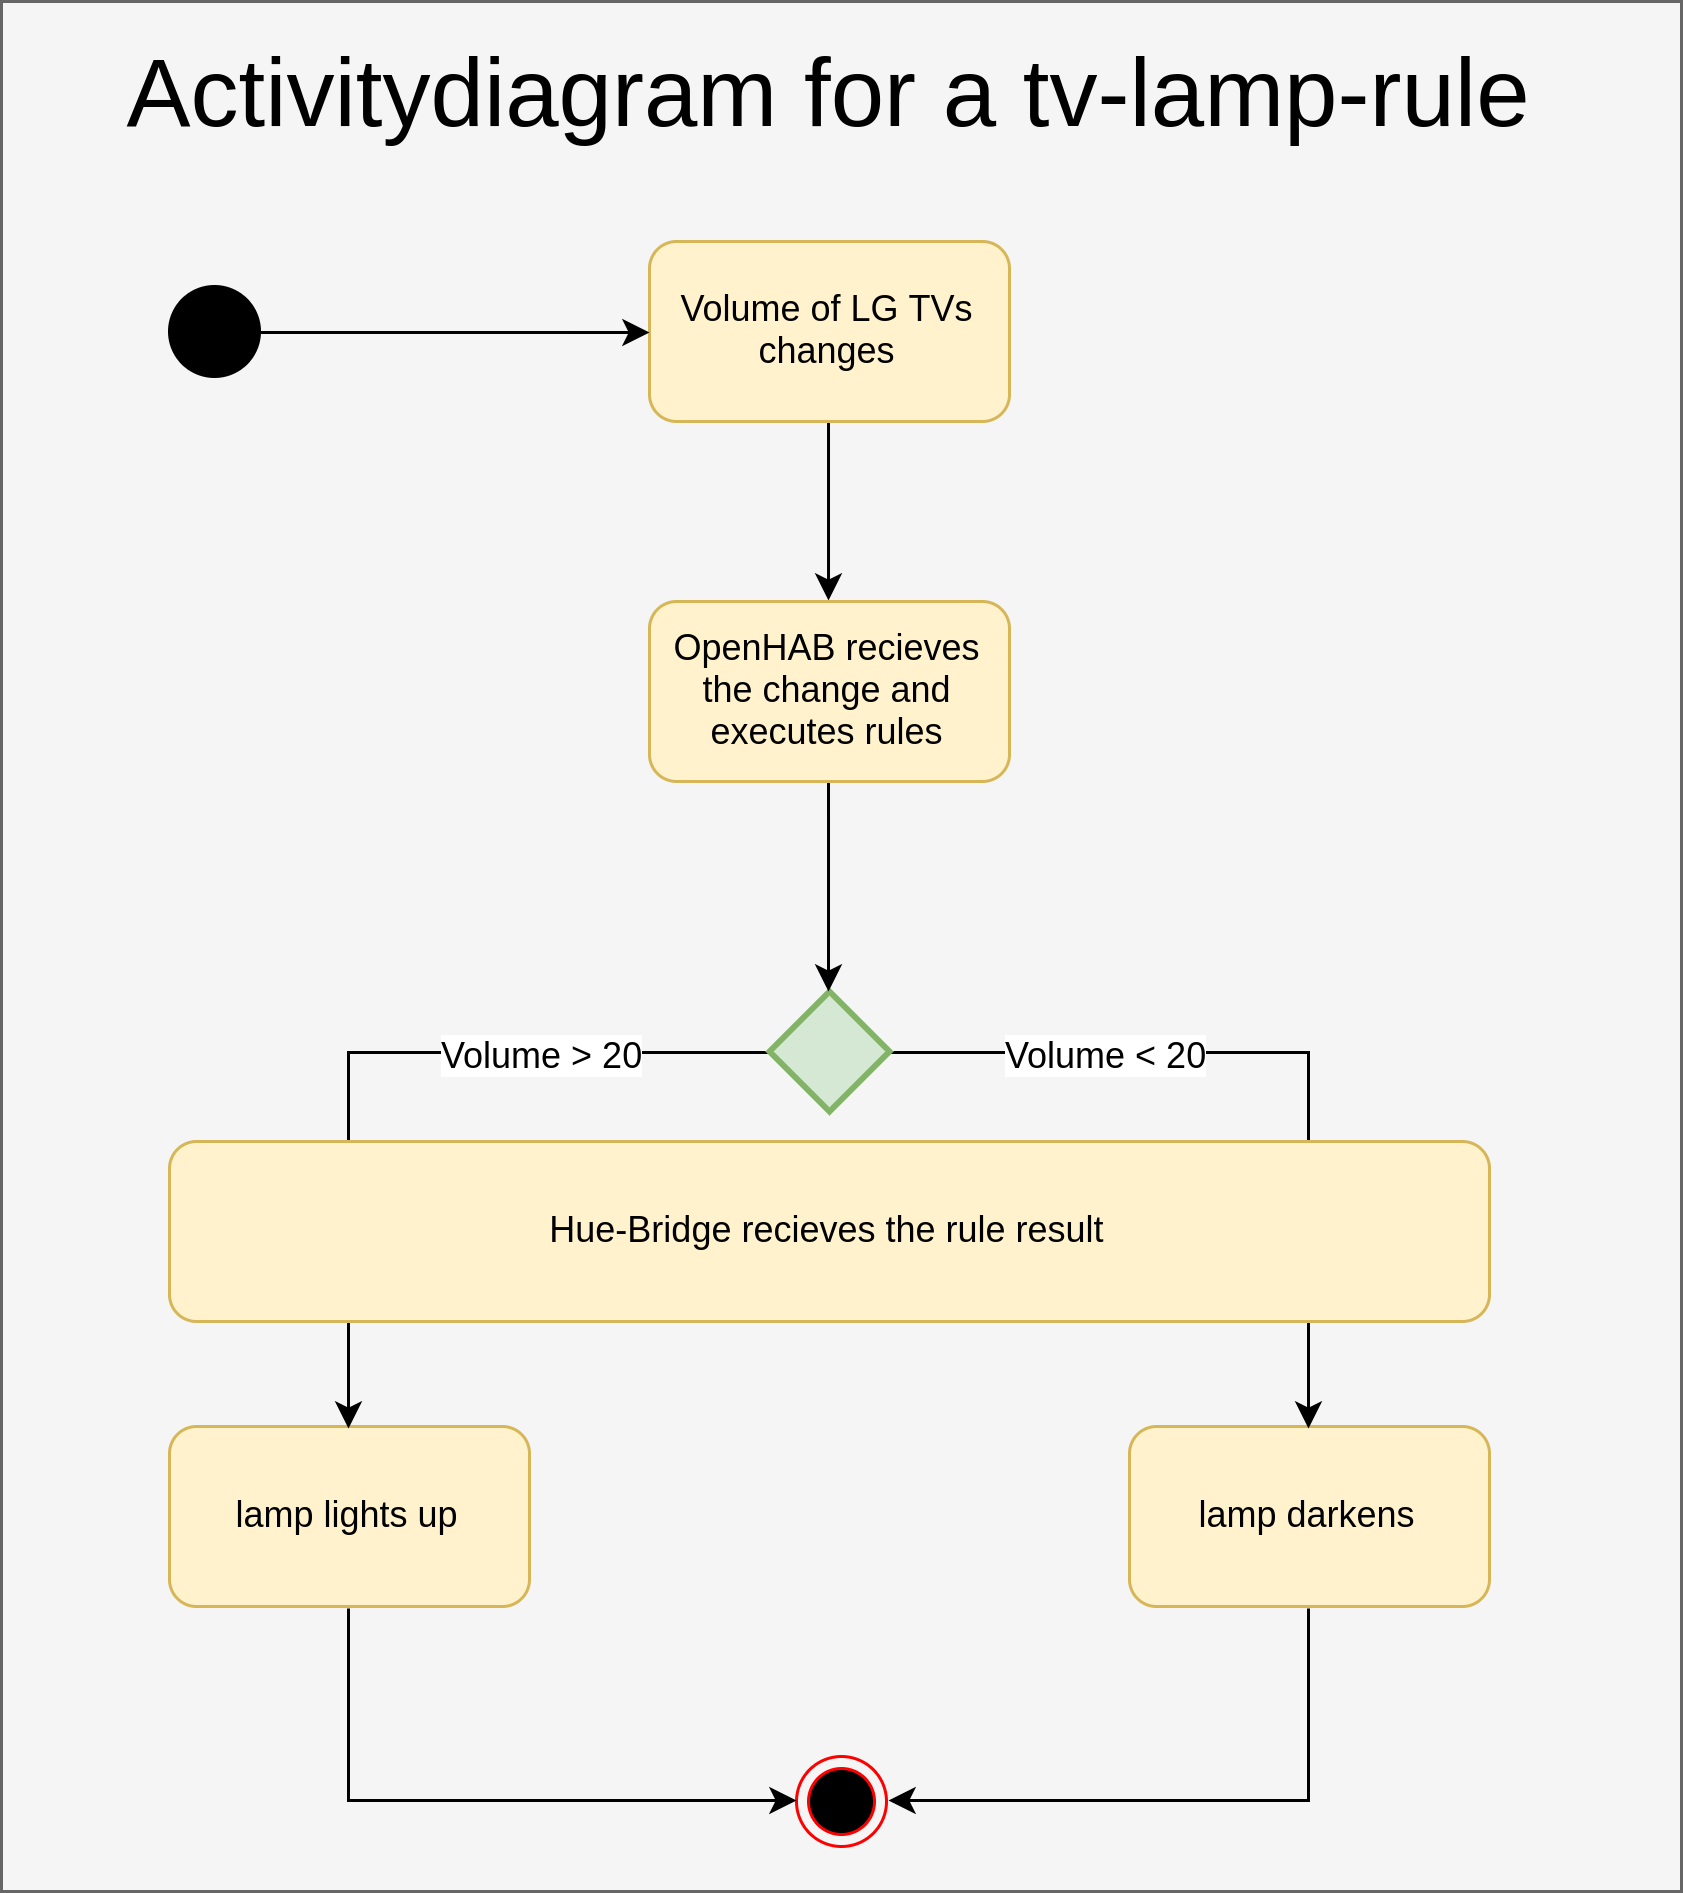
\includegraphics[width=1\textwidth]{\figdir/activitydiagram-lg-light-rule.png}
	\caption{Aktivitätsdiagram für eine Rule \label{fig:activity-diagram}}
\end{minipage}

\subsection{Umgang mit OpenHAB}
\begin{itemize}
	\item Das meiste klickt mans ich zusammen: Bindings, Rules, Channels, Items, Things
	\item Implementierung von rules scheint idiotensicher, weil:
	\begin{itemize}
		\item einfacher Syntax
		\item Abhängigkeiten managed Openhab
	\end{itemize}
	\item Bindings schreiben scheint eher schwieriger
\end{itemize}

\section{Fazit}
\subsection{Stärken}
Some of openHAB's strengths are:

Its ability to integrate a multitude of other devices and systems. openHAB includes other home automation systems, (smart) devices and other technologies into a single solution
To provide a uniform user interface and a common approach to automation rules across the entire system, regardless of the number of manufacturers and sub-systems involved
Giving you the most flexible tool available to make almost any home automation wish come true; if you can think it, odds are that you can implement it with openHAB.
\subsection{Schwächen}
\textbf{Wollen wir das hier als SWOT Analyse aufziehen?}
\begin{itemize}
	\item Integration von USB-Geräten scheint eher kompliziert. Vor allem auf Raspberry Pi
	\item Serial Binding wird nicht angezeigt
	\begin{itemize}
		\item Mikrofon an Raspberry Pi oder anderes Geräte verbinden
		\item Input des Mikrofons über OpenHAB an ein Ausgabegerät, wie zum Beispiel eine Bluetooth Box, senden und abspielen
		\item Raspberry hat da auch für große Probleme bei der Geräteerkennung gesorgt - USB gerät wurde nicht im devices Verzeichnis aufgeführt und somit konnte auch keine Verbindung mit OpenHAB aufgebaut werden
		\item OpenHAB Serial Device Binding wurde auch nicht angezeigt, um Geräte darüber zu suchen
	\end{itemize}
\end{itemize}

\section{Infos:}
\textbf{Ausgangslage}
Untersuchen Sie die Architektur und Features von OpenHAB und
schreiben Sie ein Beispielanwendung.
Mit myOpenHub existiert eine kostenlose Plattform die sie nutzen
können.

\textbf{Beantworten Sie dabei}
\begin{itemize}
 \item Aktueller Status des Projekts und  
 \item Integration der Big Player wie Alexa und Google Home
 \item Welche Tools und Konzepte und APIs gibt es
 \item Welche Deployment Modi und Betriebsmodi existieren
 \item Untersuchen Sie auch Aspekte wie Datenintegriertät und Sicherheit
\end{itemize}

\textbf{Unterlagen Linkes}
\begin{itemize}
	\item \url{https://www.myopenhab.org/}
	\item \url{https://www.openhab.org/}
	\item \url{https://jaxenter.de/openhab-2-4-78711}
\end{itemize}

%%% Local Variables: 
%%% mode: latex
%%% TeX-master: "thesis.tex"
%%% End: 
